\chapter{Comunicacion Multimedia}

\section{Enunciado}
Las aplicaciones multimedia en tiempo real permiten conectar a distintos usuarios a través de la red e intercambiando información de audio,vídeo u otro tipo de información.Un ejemplo de este tipo de aplicación es Skype que ha tenido mucho éxito ya que permite a sus usuarios establecer videollamadas e intercambiar información una vez se haya instalado el software.
\begin{figure}[!h]
\begin{center}
   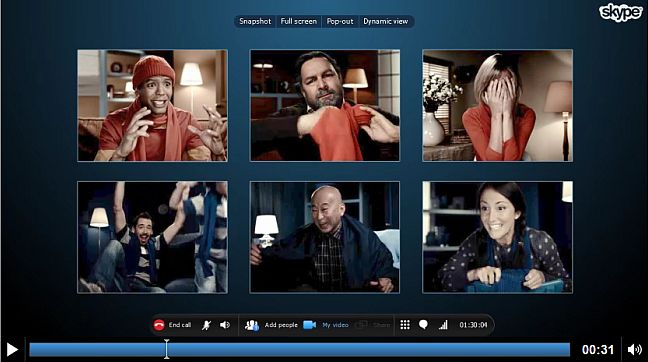
\includegraphics[width=0.9\linewidth]{Figures/skype}
	\decoRule
	\caption[Ejemplo sitio Web]{Skype interfaz videollamada.}
\label{fig:canvasPrimitivas}
\end{center}
\end{figure}
\\Por lo tanto en esta ultima practica se pide desarrollar una aplicación web similar a Skype que permita a los usuarios conectarse entre si a través de la url de la aplicación.Una vez dentro el usuario selecciona los elementos multimedia(audio y video) que desea compartir y tendrá que elegir si unirse o crear una sala donde los usuario mantendrán la comunicación.
\\Por ultimo,se podrá enviar cadena de texto entre los usuarios de una determinada sala a través del chat de la aplicación al igual que enviar archivos.

\subsection{Tecnologias necesarias}
\begin{enumerate}
\item API WebRTC
\item API File
\item NodeJS
\item Socket.io
\item JavaScript
\item Boostrap
\end{enumerate}

\subsection{Objetivos}
La practica tiene que cubrir los siguientes puntos
\begin{enumerate}
\item Creación/Unión de salas por parte de los usuarios.
\item El usuario seleccionara los elementos multimedia a compartir.
\item Transmisión de los elementos multimedia seleccionados entre los usuarios.
\item Creación de un servidor de señalizacion.
\item Topologia de comunicación en Malla.
\item Comunicación final Peer-to-Peer entre los navegadores.
\end{enumerate}
\section{Tecnologías Aplicadas}
\subsection{API File}
El tratamiento de ficheros por parte de los navegadores de forma nativa no fue posible hasta que el nuevo estándar de HTML5 incorporase API File.
\\La API requiere de una etiqueta 'input' para seleccionar el documento con el que se quiere trabajar,a continuación JavaScript se encargara de obtener la información del documento a través del objeto 'FileReader()'.
\begin{lstlisting}[
frame=single,
commentstyle=\color{CadetBlue},
captionpos=b,
caption=Ejemplo API File.]
<!DOCTYPE html>
<head>
 <meta charset="utf-8">
 <title>File API</title>
 <script type="text/javascript">
  function processFiles(file){
   var files = file[0];
   var reader = new FileReader();
   reader.onload = function (e) {
    /*
     e.result tiene el resultado de la 
     lectura del fichero
    */
   };
   reader.readAsArrayBuffer(files);
  }
 </script>
</head>
<body>
 Select a text file:
 <input type="file" id="fileInput" onchange="processFiles(this.files)">
</body>
</html>
\end{lstlisting}
Es necesario especificar el modo en el que la API va a leer la información, a continuación se resumen los métodos disponibles.
\begin{itemize}
\item \textbf{reader.readAsText():}
\\Permite leer archivos de texto y recibe dos parámetros. El primer parámetro es un objeto file o Blob que se va a leer y el segundo parámetro se utiliza para especificar la codificación del archivo.
\item \textbf{reader.readAsDataURL():}
\\Permite leer un File o Blob y generar una URL de datos . Esto es básicamente una cadena base64 de los datos del archivo. Se puede utilizar esta URL datos para cosas como el establecimiento de la src propiedad de una imagen.
\item \textbf{reader.readAsBinaryString():}
\\Permite leer cualquier tipo de archivo. El método devuelve los datos binarios sin formato.
\item \textbf{reader.readAsArrayBuffer():} 
\\Permite leer un File o Blob y obtener como resultado un ArrayBuffer,es decir,un buffer de datos binarios de longitud fija.
\end{itemize}
\subsection{GetUserMedia}
Es una herramienta por parte de los navegadores que permite acceder a los elementos multimedia de un ordenador/móvil/tablet que pueden ser el micrófono y/o la web-Cam.
\begin{lstlisting}[
frame=single,
commentstyle=\color{CadetBlue},
captionpos=b,
caption=Instancia RTCPeerConnection.]
 var items = {
  audio:true,
  video:true
 }
 navigator.getUserMedia(items,connect_items,error_items);
\end{lstlisting}
La función 'getUserMedia' recibe como parámetro los elementos a los que el navegador desea acceder a través de la variable 'items' y la función 'connect\_items' se encarga de presentar en el navegador los elementos multimedia.El tercer parámetro es la función 'error\_items' que se ejecuta cuando se produce algún fallo al acceder a los elementos.

\subsection{Servidor de Señalización (NodeJS +Socket.IO)}
Para generar un servidor utilizamos NodeJS, ya que con pocas lineas de código obtenemos un servidor el cual se encarga de suministrar a los usuarios de la pagina principal de la aplicación.
\begin{lstlisting}[
frame=single,
commentstyle=\color{CadetBlue},
captionpos=b,
caption=Instancia RTCPeerConnection.]
 var static = require('node-static');
 var http = require('http');
 var file = new(static.Server)();
 var app = http.createServer(function (req, res) {
  file.serve(req, res);
 }).listen(8181);
\end{lstlisting}
Tras esto es necesario utilizar un mecanismo de comunicación entre el cliente y el servidor, con el objetivo de enviar información acerca de la sesión de cada usuario.Por ello utilizamos socket.io que es un biblioteca de WebSocket que permite una comunicación en tiempo real entre el cliente y el servidor con baja latencia y permitiendo una comunicación bidireccional.
\\Para ello instalamos a través del interfaz de NodeJS la librería de socket.io con el comando 'npm save-- socket.io' y lo llamamos dentro del proyecto.
\begin{lstlisting}[
frame=single,
commentstyle=\color{CadetBlue},
captionpos=b,
caption=Instancia socket.io servidor.]
 var io = require('socket.io').listen(app);
\end{lstlisting}
Es necesario este tipo de servidores para encaminar los mensajes entre los distintos peers. Aunque la comunicación final se realiza Peer-to-Peer al utilizar WebRTC es necesario un intercambio previo de información entre los nodos como la descripción de sesión e información de red de cada uno de ellos ,este proceso es conocido como señalizacion.

\subsection{WebRTC}
El núcleo de la la aplicación se basa en la utilizacion del interfaz de WebRTC ya que permite establecer comunicacion entre navegadores Peer-to-Peer.El interfaz de la API se apoya en RTCPeerConnection para el establecimiento de la conexion entre los navegadores y Datachannel que permite enviar flujo de datos tras la conexion.
\subsubsection*{RTCPeerConection}
RTCPeerConection es un componente de WebRTC que permite establecer una comunicación fiable y eficiente de streamig entre peers estableciendo una comunicación Peer-to-Peer.
\\Es necesario un intercambio previo de mensajes para acordar los parámetros de la comunicación entre los nodos a través del servidor de señalizacion.Por otra parte RTCPeerConection usa en el protocolo ICE que en conjunto a los servidores STUN/TURN permite establecer la conexión a través de NAT's y firewalls.
\begin{lstlisting}[
frame=single,
commentstyle=\color{CadetBlue},
captionpos=b,
caption=Instancia RTCPeerConnection.]
 var pc = new RTCPeerConnection({
  'iceServer':[{'url':'stun:stun.l.google.com:19302'}]
 });
\end{lstlisting}
A través de la instancia se tiene acceso a los métodos de los que dispone el objeto,a continuación pasamos a explicar los métodos/eventos que se utilizaran en el desarrollo de la practica.
\begin{itemize}
\item \textbf{pc.addStream(stream):}
\\AddStream() añade un nuevo objeto MediaStream al objeto RTCPeerConnection.
\item \textbf{pc.onaddstream:}
\\Onaddstream es evento que se dispara cada vez que se añade un objeto MediaStream por el par remoto.
\item \textbf{pc.createOffert(HandlerOffert,HandlerError,Options):}
\\CreateOffert() genera un objeto SDP con la configuración de la sesión,ademas incluye la descripción del streaming local.El método recibe la función HandlerOffert que se encarga de componer el mensaje cuando el proceso ha tenido éxito mientras que la función HandlerError se ejecuta cuando se produce un error.
\item \textbf{pc.createAnswer(HandlerAnswer,HandlerError,Options):}
\\CreateAnswer() se utiliza para contestar una oferta enviada a traves de una conexion remota.Se encarga de crear un objeto SDP que sea complatible con la descripcion de sesion recibida en la oferta,ademas se incluye la descripcion del streaming local.En cuanto a los parametros que recibe el metodo sigue la misma estructura que al crear la oferta.
\item\textbf{pc.onicecandidate:}
\\Onicecandidate es evento que se dispara cuando el protocolo ICE encuentra un candidato (Ip:Puerto) que permita conectarse con un peer remoto.
\item\textbf{pc.addIcecandidate(candidate):}
\\El método addIceCandidate () proporciona un candidado al protocolo ICE,ademas se es necesario añadirlo a la descripcion remota para establecer la conexion peer-to-peer.
\item\textbf{pc.createDataChannel(etiqueta DOMString,Options):}
\\CreateDataChannel crea un objeto RTCDataChannel con la etiqueta dada,opcionalmente se puede establecer la configuracion del canal a traves de la variable options.
\item\textbf{pc.ondatachannel:}
\\Ondatachannel es un evento que se llama para incluir el canal en el par remoto.
\end{itemize}
\subsubsection*{DataChannel}
DataChannel es el ultimo de los componente que utiliza WebRTC para enviar datos entre los peers una vez la conexion se ha establecido por completo.
\\La API dota a los navegadores web de una comunicacion de datos bidireccional entre los peers,ademas soporta gran variedad de datos como Blob,ArrayBuffer y ArrayBuuferView.
\begin{lstlisting}[
frame=single,
commentstyle=\color{CadetBlue},
captionpos=b,
caption=Ejemplo creacion DataChannel.]
 var sendChannel = pc.createDataChannel('nombre_canal',opciones);
\end{lstlisting}
Tras la creacion del canal disponemos una serie de eventos que permiten trabajar con el canal que se ha establecido,a continuacion se explica cada uno de estos eventos.
\begin{itemize}
\item \textbf{sendChannel.onopen:}
\\Onopen evento que se ejecuta cuando el canal de comunicacion se encuentra disponible.
\item \textbf{sendChannel.onmessage:}
\\Onmessage evento que permite la recepcion de los datos que se son enviados a traves del canal establecido.
\item \textbf{sendChannel.onclose:}
\\Onclose evento que permite cerrar el canal.
\end{itemize}
Se partira de un ejemplo ya resuelto en el libro [WebRTC] donde la com
unicacion se realiza entre dos usuarios y transmiten flujo de audio/video entre ellos. Con el objetivo de entender el entendimiento e ir un paso mas alla se implementa los siguientes elementos.

%%%%%%%%%%%%%%%%%%%%%%%% SECCION DESARROLLO %%%%%%%%%%%%%%%%%%%%%%%%

\section{Desarrollo}
Una vez explicado el funcionamiento de las tecnologías  que se van a emplear pasamos a describir como se emplean en la realización del desarrollo.
Se va a dividir en dos partes cliente y servidor con el objetivo de explicar de forma adecuada el funcionamiento de cada parte.

%%%%%%%%%%%%%%%%%%%%%%%%%%%%%%%%%%%%%
%%%%%%%% Servidor Desarrollo %%%%%%%%
%%%%%%%%%%%%%%%%%%%%%%%%%%%%%%%%%%%%%

\subsection{Servidor de señalización}
Como se ha explicado a lo largo del capitulo es necesario establecer un servidor de señalizacion para que los peers puedan intercambien información previa al establecimiento de la comunicación.
\\El primer paso para crear el servidor es importar la libreria 'node-static','http' y 'socket.io'.La libreria 'http' permite crear un servidor a traves del metodo createServer en el puerto 8181 en nuestro caso mientras que la libreria 'node-static' permite enviar el documento a los usuarios que se conecten,este documento se llamara 'index.html'.
\\Finalmente, la libreria 'socket.io' se utiliza para establecer comunicacion entre el cliente y servidor(\textbf{fig \ref{fig:EjecucionServer}}).
\begin{lstlisting}[
frame=single,
commentstyle=\color{CadetBlue},
captionpos=b,
caption=Creacion Servidor de Señalizacion.]
 var static = require('node-static');
 var http = require('http');
 var file = new(static.Server)();
 var app = http.createServer(function (req, res) {
  file.serve(req, res);
 }).listen(8181);
 var io = require('socket.io').listen(app);
\end{lstlisting}
\begin{figure}[!h]
\begin{center}
   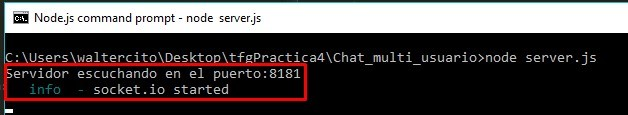
\includegraphics[width=0.6\linewidth]{Figures/InicioServidor}
	\decoRule
	\caption[ServidorSeñalizacion]{Ejecucion Servidor de Señalizacion APP.}
\label{fig:EjecucionServer}
\end{center}
\end{figure}
El siguiente paso es permitir al servidor gestionar adecuadamente cada conexión que se establece a través de socket.io.Por ello, a través del método 'conected' mantendremos conectado.
\\El primer mensaje que recibe el servidor es 'InfoRoom' que realiza una peticion de las salas disponibles.A esta peticion el servidor contesta con un mensaje 'ReplayInfoRoom' con la lista de las salas en la variable 'listRoom'(\textbf{fig \ref{fig:EjecucionInfoRoom}}).
\begin{lstlisting}[
frame=single,
commentstyle=\color{CadetBlue},
captionpos=b,
caption=Request/Replay lista de salas existentes.]
 socket.on('infoRoom',function(name) {
  socket.emit('ReplayInfoRoom',listRooom);
 });
\end{lstlisting}
\begin{figure}[!h]
\begin{center}
   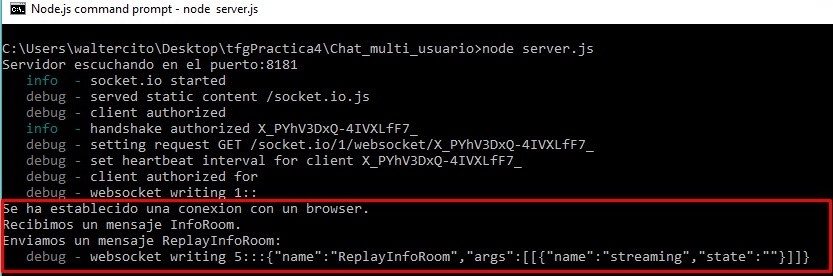
\includegraphics[width=0.6\linewidth]{Figures/InfoRoomServer}
	\decoRule
	\caption[Request/Replay Salas Servidor]{Request/Replay lista de salas del Servidor.}
\label{fig:EjecucionInfoRoom}
\end{center}
\end{figure}
Tras el envió de la lista de salas disponibles el servidor recibirá un mensaje 'Stablish\_connect' con el nombre y sala a la que desea conectarse.Se comprueba si el nombre de sala existe o no a través de la función 'getRoom(nameRoom)' en caso de no existir se guardara en la lista con la función 'setRoom()'.
\\Tras esta comprobación pasamos a comprobar el numero de usuarios existente en la sala a través de 'io.sockets.clients(room).length' .
\\Si la sala no esta completa el servidor envía un mensaje 'CreateStream' con el identificador de conexión al usuario que ha solicitado entrar en la sala y un mensaje' NewJoined' al resto de usuario de la sala para que conozcan la existencia del nuevo miembro (\textbf{fig \ref{fig:EjecucionStablishConnection}}).
\begin{lstlisting}[
frame=single,
commentstyle=\color{CadetBlue},
captionpos=b,
caption=Request/Replay del establecimiento de conexion.]
 socket.on('stablish_connection',function(name,room){
  /*comprobamos la existencua de la sala */
  if(!getRoom(room)){
    setRoom(room,'');
  };
  /* comprobamos el numero de usuarios */
  var numClients = io.sockets.clients(room).length;
  if(numClients < 3){
   socket.username = name;
   socket.room =room;
   socket.join(room);
   socket.emit('CreateStream',socket.id);
   socket.broadcast.to(room).emit('New_Joined',socket.id);
  }else{
   socket.emit('RejectStream',socket.id);
  }
 });
\end{lstlisting}
\begin{figure}[!h]
\begin{center}
   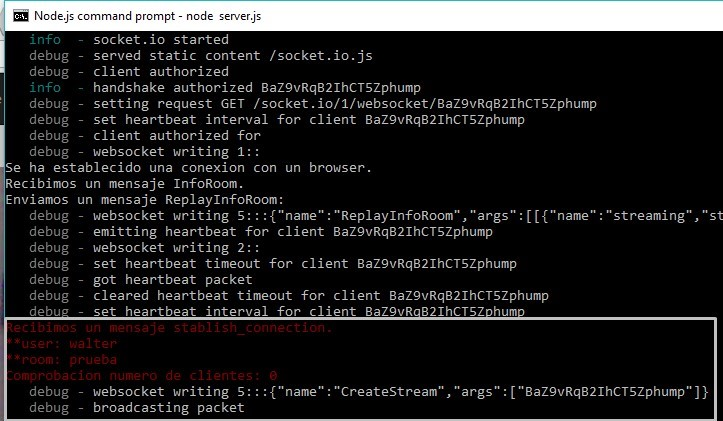
\includegraphics[width=0.6\linewidth]{Figures/StablishConnectionServer}
	\decoRule
	\caption[Request/Replay conexión Servidor]{Request/Replay conexión al Servidor.}
\label{fig:EjecucionStablishConnection}
\end{center}
\end{figure}
Por ultimo, tras haber enviado el mensaje 'New\_Joined' los usuarios empiezan el proceso de señalizacion generando mensajes de tipo 'message' con id del cliente destino para que el servidor encamine correctamente el mensaje.
\begin{lstlisting}[
frame=single,
commentstyle=\color{CadetBlue},
captionpos=b,
caption=Mensajes de señalizacion.]
 socket.on('message',function(message,room){
  io.sockets.socket(message.id_dest).emit('message', message);
 });
\end{lstlisting}
\begin{figure}[!h]
\begin{center}
   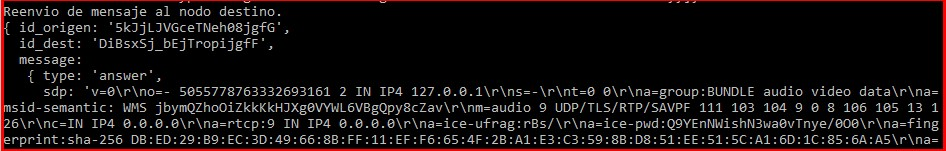
\includegraphics[width=0.8\linewidth]{Figures/AnswerServer}
	\decoRule
	\caption[Request/Replay conexión Servidor]{Mensaje tipo Answer.}
\label{fig:EjecucionStablishConnection}
\end{center}
\end{figure}
\begin{figure}[!h]
\begin{center}
   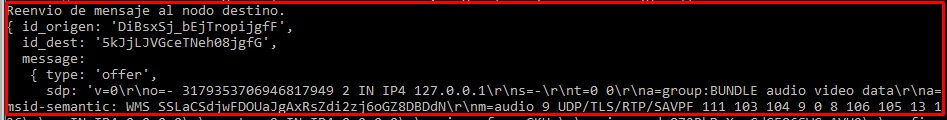
\includegraphics[width=0.8\linewidth]{Figures/OfferServer}
	\decoRule
	\caption[Request/Replay conexión Servidor]{Mensaje tipo Offer.}
\label{fig:EjecucionStablishConnection}
\end{center}
\end{figure}
\begin{figure}[!h]
\begin{center}
   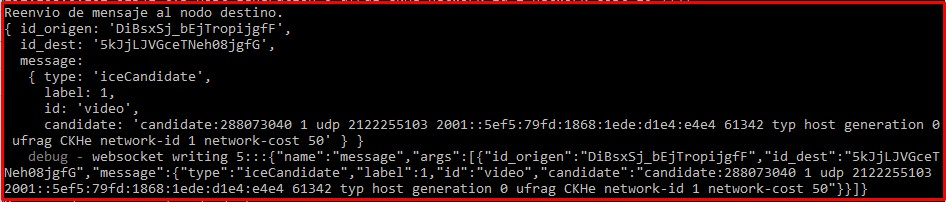
\includegraphics[width=0.8\linewidth]{Figures/IceCandidateVideos}
	\decoRule
	\caption[Request/Replay conexión Servidor]{Mensaje tipo Icecandidate.}
\label{fig:EjecucionStablishConnection}
\end{center}
\end{figure}
El servidor deja de participar en el intercambio de información entre los peers cuando el proceso de señalizacion termina ya que desde ese momento la comunicación es Peer-to-Peer.

%%%%%%%%%%%%%%%%%%%%%%%%%%%%%%%%%%%%
%%%%%%%% Cliente Desarrollo %%%%%%%%
%%%%%%%%%%%%%%%%%%%%%%%%%%%%%%%%%%%%

\subsection{Cliente}
Los usuarios se conectan al servidor a través de un navegador el cual recibe la pagina principal de la aplicación y este ejecuta la lógica del cliente.
\\Se establece la conexión con el servidor a través de Websockets y se pide al usuario que introduzca el nombre que utilizara en la aplicación para poder acceder al contenido de la aplicación.
\begin{lstlisting}[
frame=single,
commentstyle=\color{CadetBlue},
captionpos=b,
caption=Instancia WebSockect en el cliente.]
 var socket = io.connect("http://localhost:8181");
\end{lstlisting}
Cuando el usuario accede a la aplicación enviamos un mensaje 'infoRoom' a través de la instancia de WebSockets al servidor para obtener la lista de salas creadas\textbf{(fig \ref{fig:SelectItemsClient})}.
\begin{lstlisting}[
frame=single,
commentstyle=\color{CadetBlue},
captionpos=b,
caption=Petición salas disponibles.]
 socket.emit('infoRoom');
\end{lstlisting}
El servidor contesta con un mensaje 'ReplayInfoRoom' con la información solicitada\textbf{(fig \ref{fig:SelectItemsClient})}.
\begin{lstlisting}[
frame=single,
commentstyle=\color{CadetBlue},
captionpos=b,
caption=Creación desplegable de salas.]
 socket.on('ReplayInfoRoom',function(listRoom){
  for(var i = 0; i < listRoom.length; i++) {
   var room = listRoom[i];
   $('#listRoom').append('<li><a id='+room.name+'>'+room.name+'</a></li>');
   $('#'+room.name).click(function(){
     nameRoom = $(this).text();
     attachmentElements();
   });
  }
 });
\end{lstlisting}
A continuación, el usuario dispone en la barra de navegación de la posibilidad de seleccionar los elementos que desea compartir\textbf{(fig \ref{fig:SelectItemsClient})}.
\begin{figure}[!h]
\centering
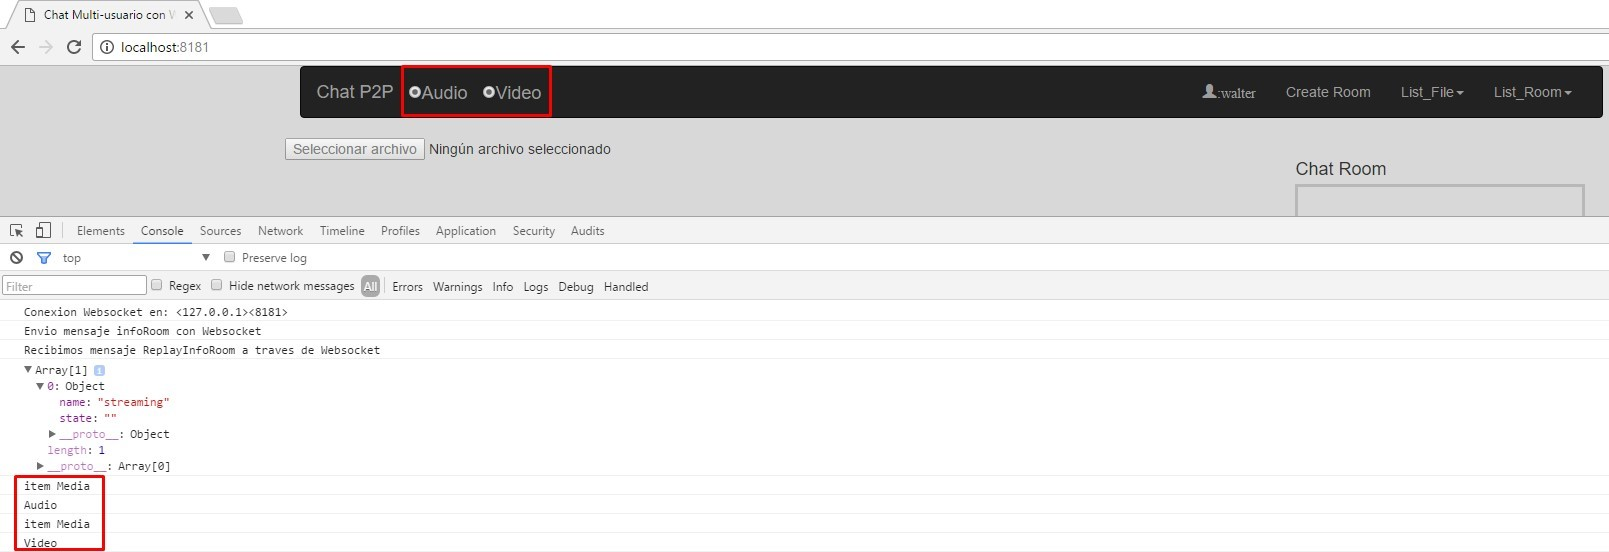
\includegraphics[width=0.7\linewidth]{Figures/SelectItemsClient}
\decoRule
\caption[An Electron]{ComunnicacionWebRTC (artist's impression).}
\label{fig:SelectItemsClient}
\end{figure}
\\Una vez los elementos han sido seleccionados el usuario puede unirse a una de las salas existentes o crear una nueva sala.En cualquiera de estas opciones se envía un mensaje 'stablish\_conection'con el nombre del usuario y el de la sala a la que desea conectarse(\textbf{fig \ref{fig:StablishConnectionClient}}).
\begin{lstlisting}[
frame=single,
commentstyle=\color{CadetBlue},
captionpos=b,
caption=envio mensaje inicio conexion.]
 socket.emit('stablish_connection',name,nameRoom);
\end{lstlisting}
Como respuesta al mensaje el servidor contesta al cliente original con un mesaje 'CreateStream' si el proceso se ha realizado correctamente(\textbf{fig \ref{fig:StablishConnectionClient}}).
\begin{lstlisting}[
frame=single,
commentstyle=\color{CadetBlue},
captionpos=b,
caption=recepción contestación elementos inicio conexión.]
 socket.on('CreateStream',function(id){
  my_id = id;
 });
\end{lstlisting}
\begin{figure}[!h]
\centering
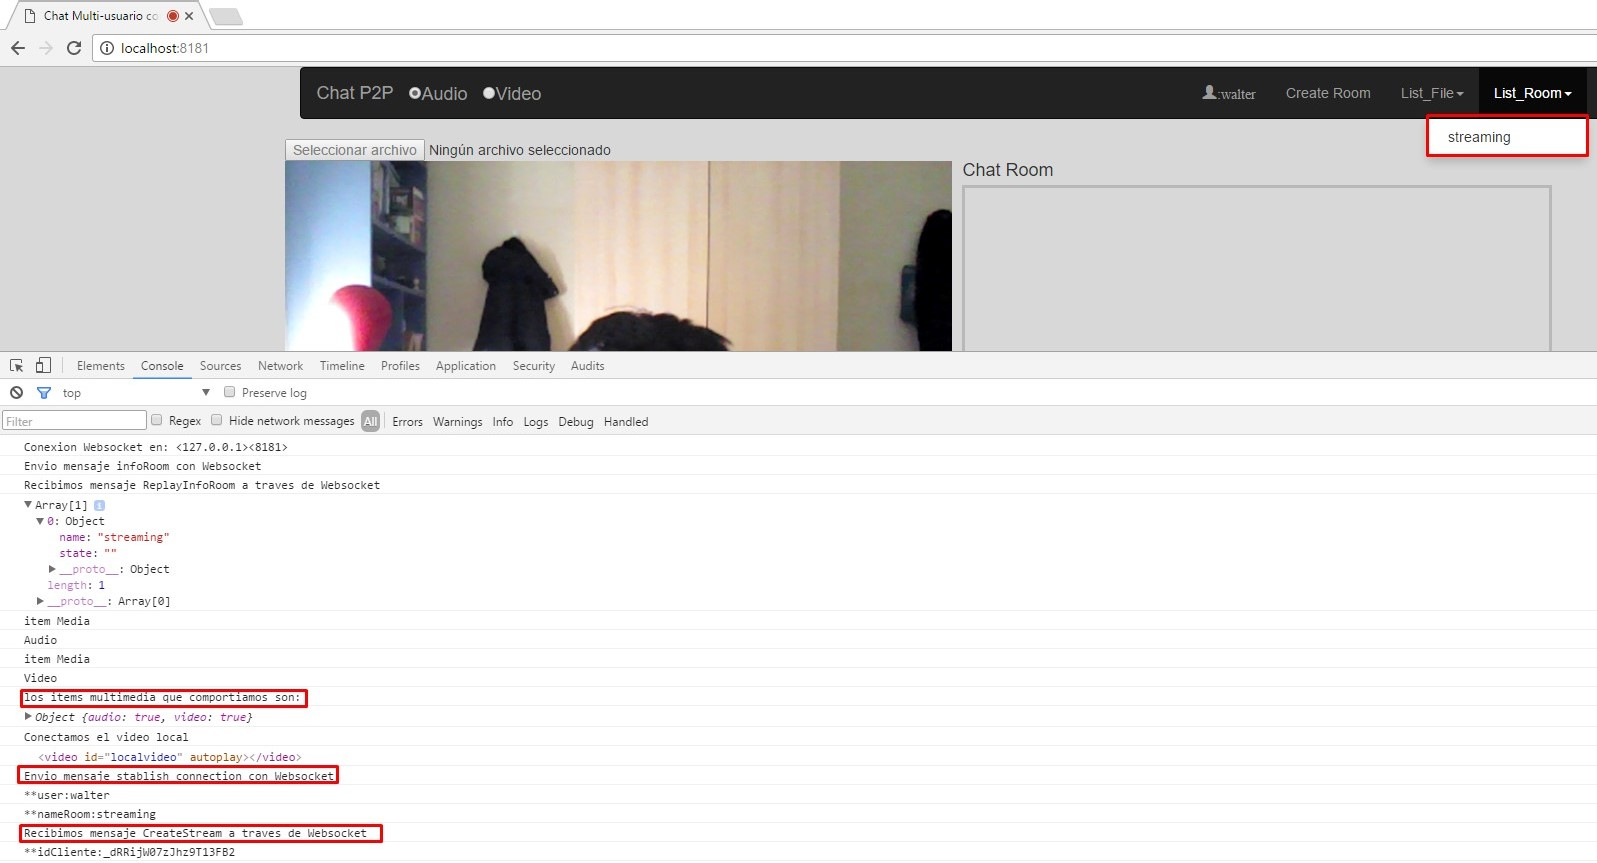
\includegraphics[width=0.7\linewidth]{Figures/StablishConnectionClient}
\decoRule
\caption[An Electron]{ComunnicacionWebRTC (artist's impression).}
\label{fig:StablishConnectionClient}
\end{figure}
Mientras que los demás usuarios recibirán el mensaje 'New\_Joined' con el identificador asociado al usuario que ha solicitado la conexión.
\begin{lstlisting}[
frame=single,
commentstyle=\color{CadetBlue},
captionpos=b,
caption=Incluir elementos multimedia remotos l.]
 socket.on('New_Joined',function(id){
  id_newUser = id;
  create_connection(id_newUser);
 });
\end{lstlisting}
A partir de este mensaje empieza el proceso de señalizacion por parte de los usuarios que han recibido el mensaje. Este proceso se divide en tres etapas:
Offert,Answer y Icecandidate.

%%%%%%%% Cliente offert %%%%%%%%

\subsubsection{Offert}
La función 'create\_connection' recibe el identificador del nuevo cliente e inicia la creación de la oferta.Primero definimos la configuración del  protocolo ICE mediante la variable 'pc\_config' y generamos instancia del objeto RTCPeerConnection() que se almacena en la variable 'pc'.
\begin{lstlisting}[
frame=single,
commentstyle=\color{CadetBlue},
captionpos=b,
caption=Instancia RTCPeerConnection.]
 var pc_config = {'iceServers': [{'url': 'stun:stun.l.google.com:19302'}]};
 var pc = new RTCPeerConnection(pc_config,{});
 var num_user = 'user_'+ list_user.length;
 new_remote(num_user);
\end{lstlisting}
Tras esto,es necesario generar una nueva etiqueta de vídeo para visualizar el vídeo remoto una vez establecida la conexión.
\begin{lstlisting}[
frame=single,
commentstyle=\color{CadetBlue},
captionpos=b,
caption=Creación tag vídeo remoto.]
function new_remote(num_user){
 $('#list_remote').append('<video id='+num_user+'></video');
}
\end{lstlisting}
A continuación, por medio de la variable 'pc' accedemos al método 'addStream()' al que le pasamos el flujo de vídeo local y al evento 'onaddstream' que se encargara de presentar el flujo de vídeo remoto cuando este preparado(\textbf{fig \ref{fig:OfferCliente}}).
\begin{lstlisting}[
frame=single,
commentstyle=\color{CadetBlue},
captionpos=b,
caption=Vinculamos vídeo local/remoto a RTCPeerConnection.]
 /* video local */
 pc.addStream(streaming);
 /*  video remoto*/
 pc.onaddstream = function(event){
  var video = document.querySelector('#'+num_user);
  video.mozSrcObject = event.stream;
  video.play();
 };
\end{lstlisting}
El siguiente paso es definir el canal de comunicación de datos a través del método 'pc.createDataChannel' al que se le pasa el nombre del canal y definimos los eventos necesarios para manejar los mensajes(\textbf{fig \ref{fig:DataChannelOffert}}).
\begin{lstlisting}[
frame=single,
commentstyle=\color{CadetBlue},
captionpos=b,
caption=Instancia de DataChannel.]
 /* canal de datos */
 var sendChannel = pc.createDataChannel("sendDataChannel",{reliable: true})
 /* guardamos el canal */
 list_send.push(sendChannel);	
 /* eventos manejo de datos */
 sendChannel.onopen = ChannelOpen;
 sendChannel.onclose = ChannelClose;
 sendChannel.onmessage = ChannelReceive;
\end{lstlisting}
\begin{figure}[!h]
\centering
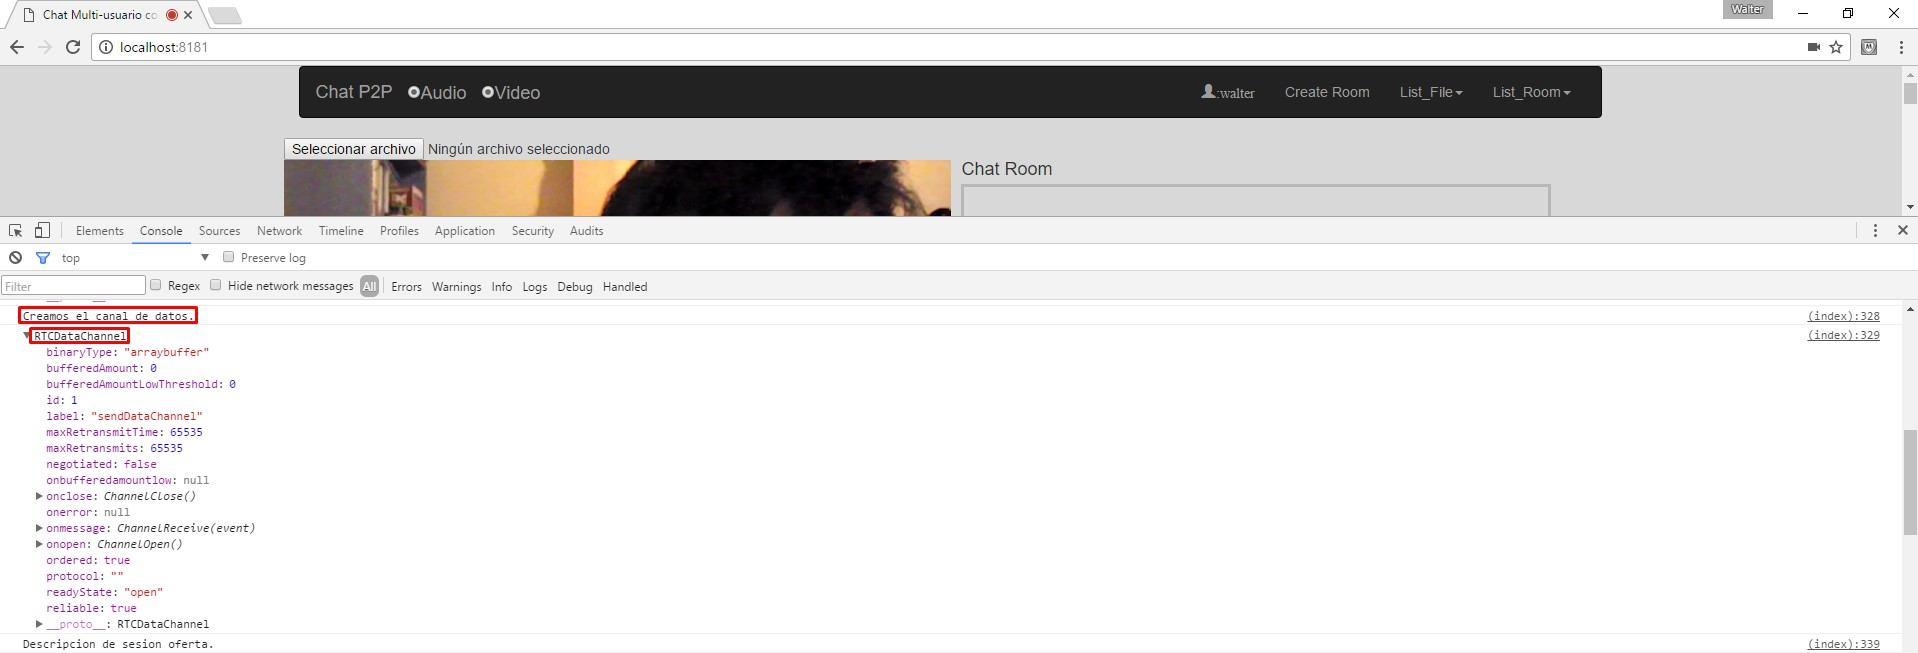
\includegraphics[width=0.7\linewidth]{Figures/DataChannelOffert}
\decoRule
\caption[An Electron]{ComunnicacionWebRTC (artist's impression).}
\label{fig:DataChannelOffert}
\end{figure}
Finalmente, definimos el método 'pc.createOffer()' en el que guardamos la descripción de sesión local con el método 'pc.setLocalDescription(sessionDescription)' y enviamos un mensaje tipo 'message' donde el cuerpo del mensaje es la oferta generada(\textbf{fig \ref{fig:OfferCliente}}).
\begin{lstlisting}[
frame=single,
commentstyle=\color{CadetBlue},
captionpos=b,
caption=Creación de la oferta.]
 pc.createOffer(function(sessionDescription){
  //guardamos esto en nuestra session
  pc.setLocalDescription(sessionDescription);
  //enviamos nuestra descripcion al nuevo usuario
  var message = create_msg(my_id,id_newUser,sessionDescription);
  socket.emit('message',message);
 },function(err){console.log(err);},{});
\end{lstlisting}
\begin{figure}[!h]
\centering
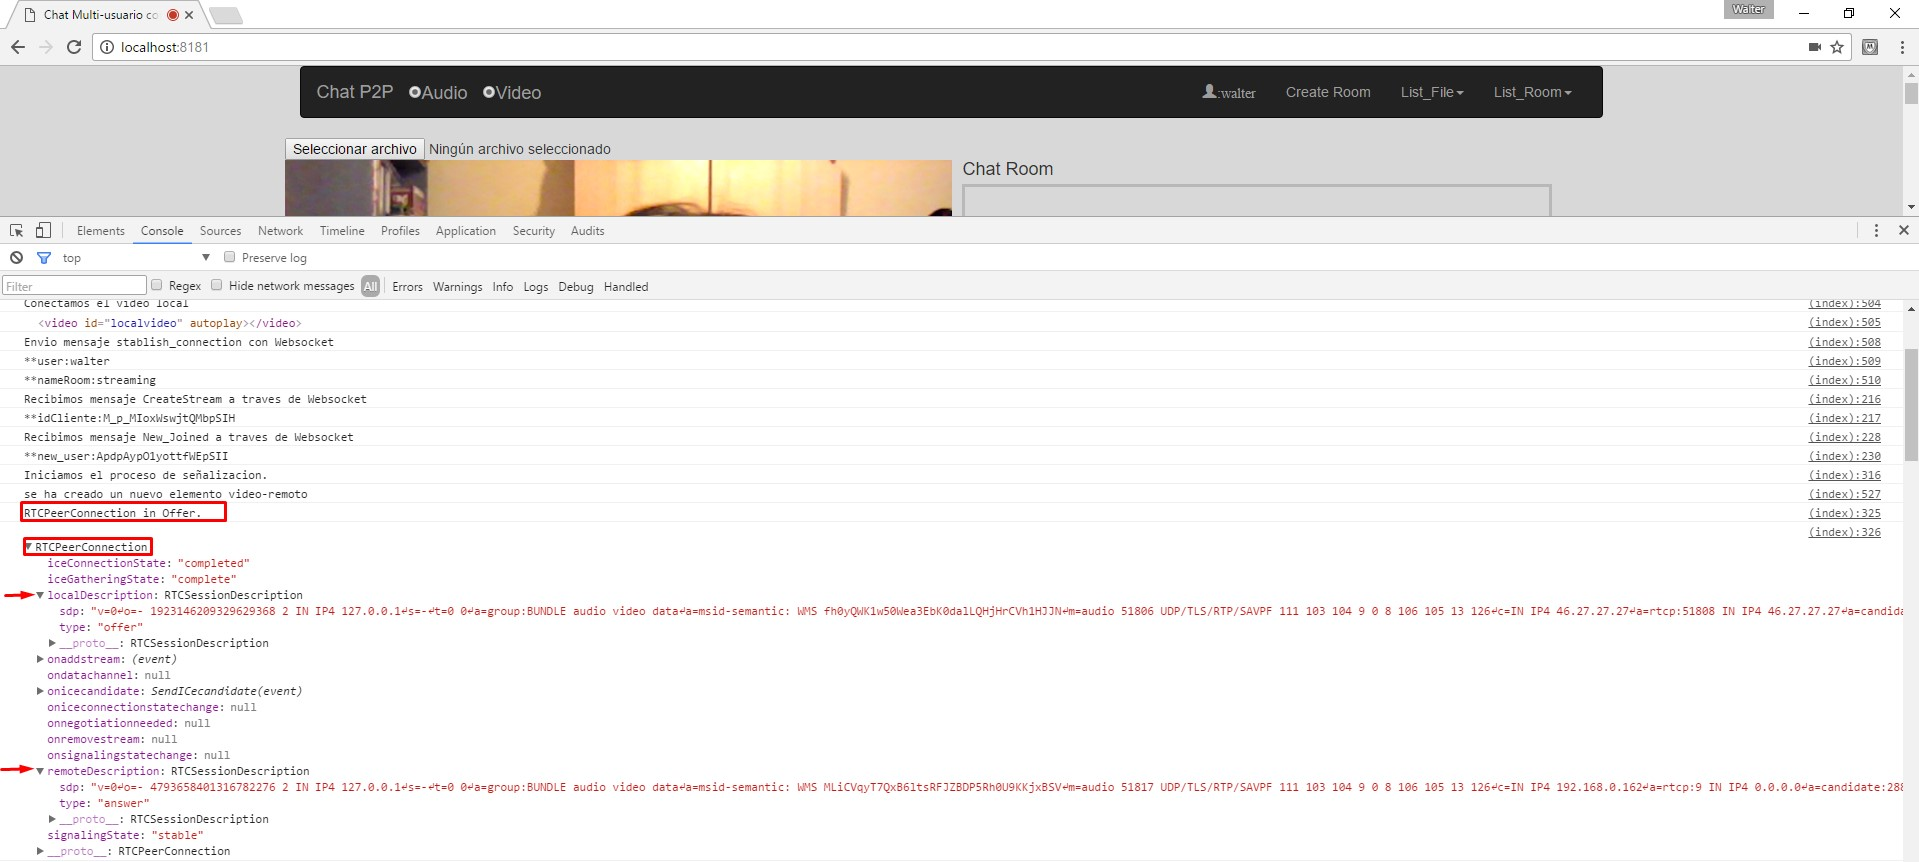
\includegraphics[width=0.7\linewidth]{Figures/OfferCliente}
\decoRule
\caption[An Electron]{ComunnicacionWebRTC (artist's impression).}
\label{fig:OfferCliente}
\end{figure}

%%%%%%%% Cliente Answer %%%%%%%%

\subsubsection{Answer}
El cliente que origina la oferta recibe un mensaje de tipo 'message' en el que evaluamos el subtipo de mensaje ya que a través de este tipo de mensaje recibimos los distintos tipos de mensaje de señalizacion.
\\Al principio generamos una instancia de RTCPeerconection() de la misma forma que se realizo en la oferta.A continuación,con la información recibida se genera un nuevo objeto RTCSessionDescription y lo guardamos como descripción de sesión remota a través del método 'setRemoteDescription()'. 
\begin{lstlisting}[
frame=single,
commentstyle=\color{CadetBlue},
captionpos=b,
caption=Guardar descripción de sesión remota.]
 pc.setRemoteDescription(new RTCSessionDescription(message.message));
\end{lstlisting}
El siguiente paso es establecer el canal de comunicación que en este caso tenemos que utilizar el evento 'ondatachannel' ya que solo se puede crear un canal de comunicación entre dos nodos y el creador de la oferta lo ha creado.De igual forma que en la oferta creamos las funciones para los eventos del canal(\textbf{fig \ref{fig:DataChannelAnswer}}). 
\begin{lstlisting}[
frame=single,
commentstyle=\color{CadetBlue},
captionpos=b,
caption=Creacion de canal de recepcion de datos.]
 pc.ondatachannel = function(event){
  list_send.push(event.channel);
  var receiveChannel = event.channel;
  /* evento de recepcion */
  receiveChannel.onmessage = ChannelReceive;
  receiveChannel.onopen = ChannelOpen;
  receiveChannel.onclose = ChannelClose;
 }
\end{lstlisting}
\begin{figure}[!h]
\centering
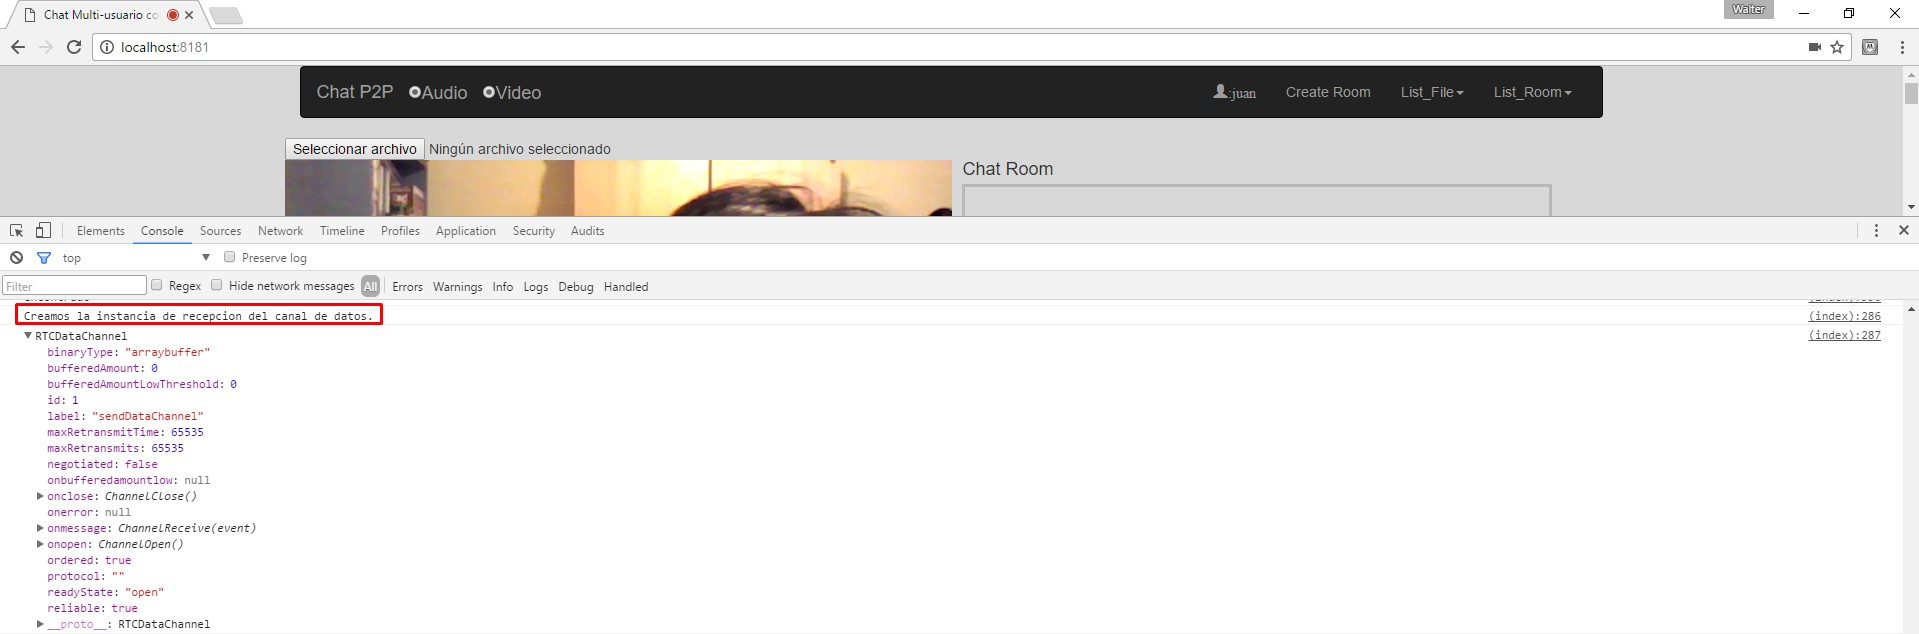
\includegraphics[width=0.7\linewidth]{Figures/DataChannelAnswer}
\decoRule
\caption[An Electron]{ComunnicacionWebRTC (artist's impression).}
\label{fig:DataChannelAnswer}
\end{figure}
Finalmente,creamos la respuesta a la oferta a través del método 'createAnswer()' dentro del cual guardaremos la información de nuestra propia sesión a través del método 'setLocalDescription' y enviamos un mensaje de tipo 'message' con la información de la sesión local para que el nodo remoto guarde esta información.
\begin{lstlisting}[
frame=single,
commentstyle=\color{CadetBlue},
captionpos=b,
caption=Creación de la respuesta.]
 pc.createAnswer(function(sessionDescription){
  pc.setLocalDescription(sessionDescription);
  var msg = create_msg(my_id,message.id_origen,sessionDescription);
  socket.emit('message',msg);
 },function(err){console.log(err);},{});
\end{lstlisting}
\begin{figure}[!h]
\centering
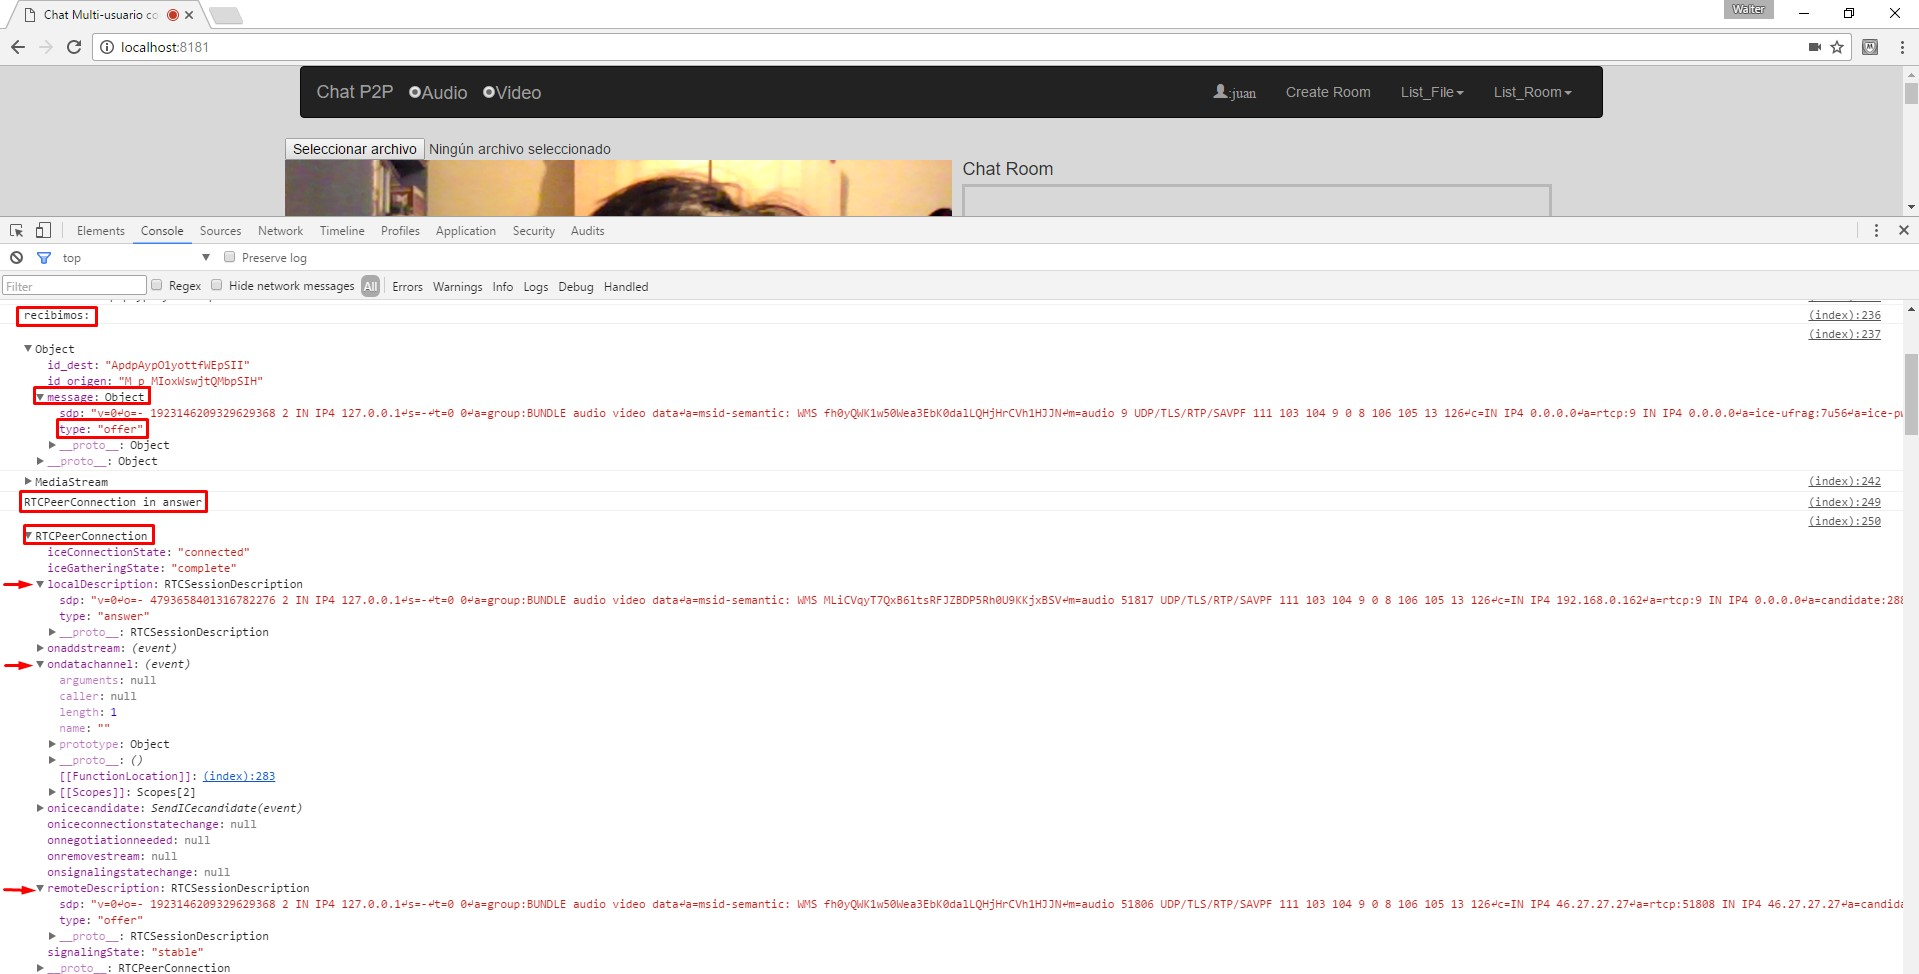
\includegraphics[width=0.7\linewidth]{Figures/AnswerCliente}
\decoRule
\caption[An Electron]{ComunnicacionWebRTC (artist's impression).}
\label{fig:Conexcion_finish}
\end{figure}

%%%%%%%% Cliente IceCandidate %%%%%%%%

\subsubsection{Icecandidate}
Tanto el usuario local y como el remoto tras la generación del objeto 'RTCPeerconnectio()' necesitan obtener información de la Ip:Puerto disponibles para la conexión por lo que se apoya en el protocolo ICE.
\\Cuando se encuentra un candidato se ejecuta el evento 'onicecandidate' que compone el mensaje con la información red  y lo envía a través de un mensaje de tipo 'message'.
\begin{lstlisting}[
frame=single,
commentstyle=\color{CadetBlue},
captionpos=b,
caption=Envio candidatos.]
 pc.onicecandidate = SendICecandidate;
 ...............
 function SendICecandidate(event){
  if(event.candidate){
   var ice = {type: 'iceCandidate',
    label: event.candidate.sdpMLineIndex,
    id: event.candidate.sdpMid,
    candidate: event.candidate.candidate
   };
   var msg ={id_origen:my_id,id_dest:id_newUser,message:ice}
   socket.emit('message',msg);
  }
}
\end{lstlisting}
Los usuarios que reciben la información anterior generan un objeto RTCIceCandidate() y se llama a la función addIcecandidate que se encarga buscar dentro de la lista de conexiones la correspondiente y asi guardar el objeto creado a través del método 'addIceCandidate'.
\begin{lstlisting}[
frame=single,
commentstyle=\color{CadetBlue},
captionpos=b,
caption=Recepcion de candidatos.]
 var candidate = new RTCIceCandidate({sdpMLineIndex:message.message.label,
  candidate:message.message.candidate
 });
 addIceCandid(message.id_origen,candidate);
 .............
 function addIceCandid(id,message){
  for(var i=0;i<list_user.length;i++){
   var user = list_user[i];
   if(user.id == id){
    user.peer.addIceCandidate(message);
   }
  }
 }
\end{lstlisting}
Una vez finalizado el proceso de señalizacion la comunicación pasa a ser Peer-to-Peer entre los clientes de una sala.(\textbf{fig \ref{fig:Coneccion_finish}}).
\begin{figure}[!h]
\centering
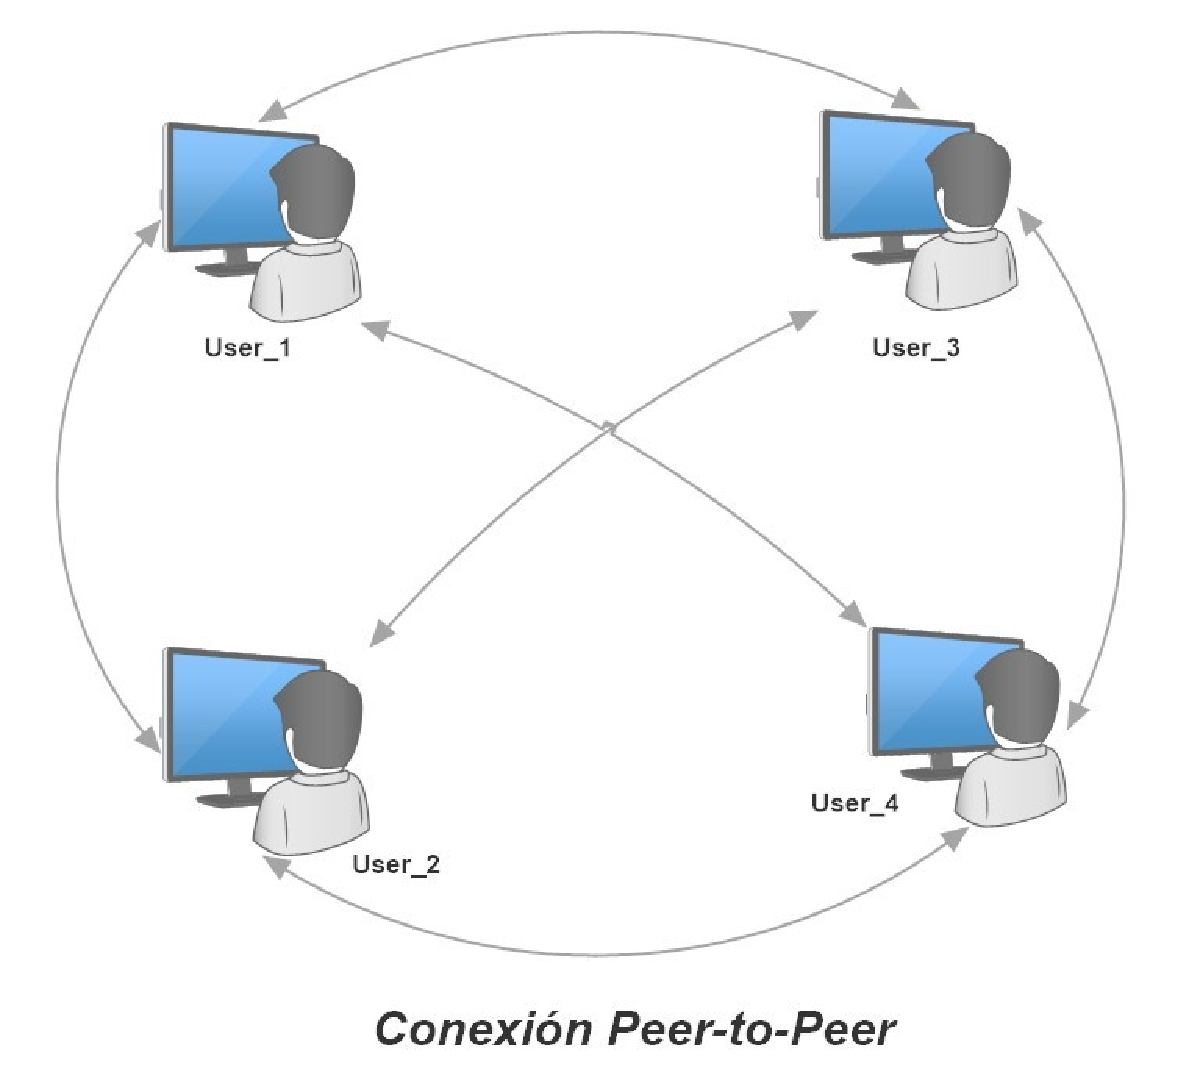
\includegraphics[width=0.6\linewidth]{Figures/Conexcion_finish}
\decoRule
\caption[An Electron]{ComunnicacionWebRTC (artist's impression).}
\label{fig:Coneccion_finish}
\end{figure}
\\Cuando la comunicación pasa a ser Peer-to-Peer se habré el canal de comunicación a través del cual enviaremos dos tipos de datos entre los usuarios.
\subsubsection{Envió de cadena de texto}
A través del chat de la sala se puede enviar cadena de caracteres entre los usuarios de la sala mediante la función 'send\_data()'.La función se encarga de obtener los caracteres que el usuario a tecleado y genera un mensaje que contiene el flag 'chat' y el dato obtenido mediante el canal de comunicación(\textbf{fig \ref{fig:ChatClienteSend}}).
\begin{lstlisting}[
frame=single,
commentstyle=\color{CadetBlue},
captionpos=b,
caption=Envió datos del chat.]
function send_data(elemento){
  var msg = $(elemento).val();
  var data = JSON.stringify({info:'chat',data:name+':'+msg});
  for(var i=0;i<list_send.length;i++){
   var user = list_send[i];
   user.send(data);
  }
  $(elemento).val('');
}
\end{lstlisting}
\begin{figure}[!h]
\centering
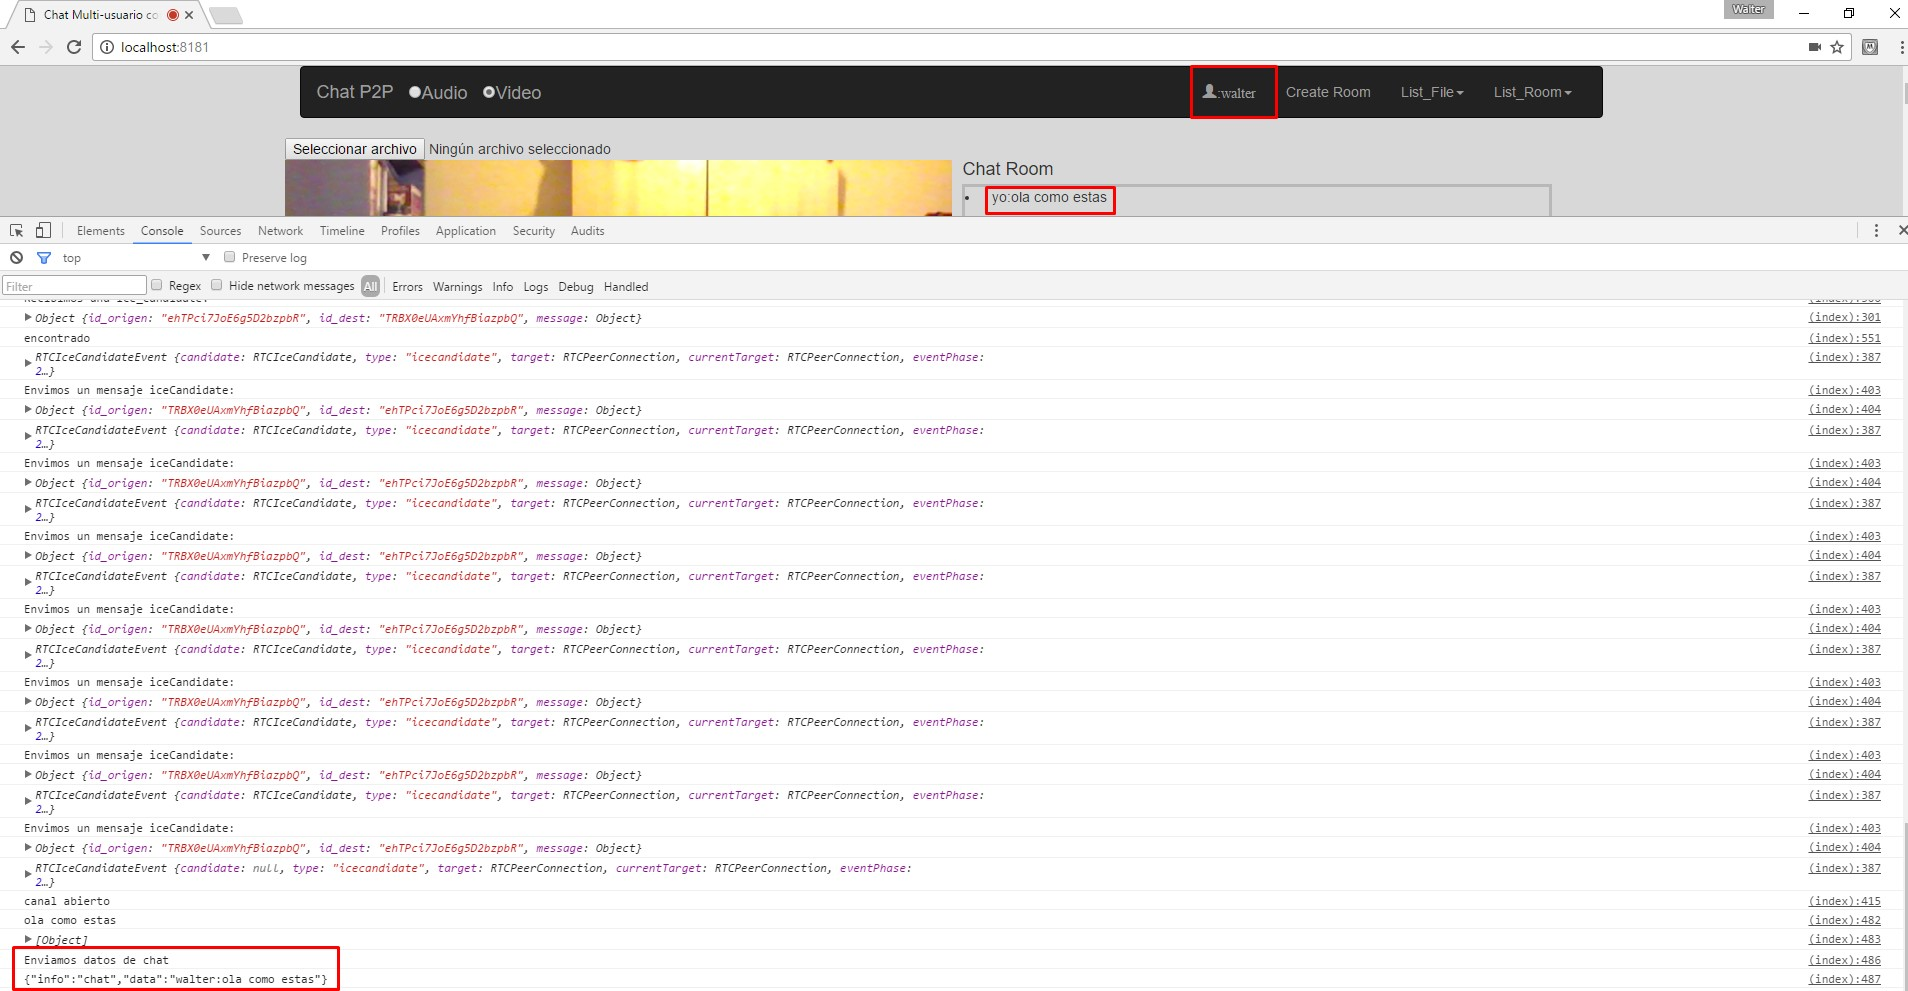
\includegraphics[width=0.8\linewidth]{Figures/ChatClienteSend}
\decoRule
\caption[An Electron]{ComunnicacionWebRTC (artist's impression).}
\label{fig:ChatClienteSend}
\end{figure}
La recepción por parte de los usuarios se realiza por medio de la función 'WriteChat(\_data)' que se encarga de presentar dentro del chat la información que se ha recibido.
\begin{lstlisting}[
frame=single,
commentstyle=\color{CadetBlue},
captionpos=b,
caption=Recepción datos del fichero.]
function WriteChat(_data){
 var line = document.createElement('li');
 var textnode = document.createTextNode(_data.data);
 line.appendChild(textnode);
 $('#texto').append(line);
}
\end{lstlisting}
\subsubsection{Envió de ficheros}
Los usuarios disponen de un 'input' de tipo file con el que carga el fichero que desea compartir.Tras seleccionar el fichero se ejecuta la función 'processFiles(file)' para obtener el contenido del fichero a través del objeto 'FileReader()' estableciendo como modo de lectura 'readAsArrayBuffer(file)'(\textbf{fig \ref{fig:fildSendUser}}). 
\begin{lstlisting}[
frame=single,
commentstyle=\color{CadetBlue},
captionpos=b,
caption=Lectura del fichero.]
 function processFiles(file){
  var files = file[0];
  type = files.type;
  name_fich = files.name;
  var reader = new FileReader();
  reader.onload = function (e) {
   var data_file = reader.result;
   data_encript = arrayBufferToBase64(data_file);
   send_chucky();
  };
  reader.readAsArrayBuffer(files);
 }
\end{lstlisting}
El envió de los datos se realiza por medio de la función 'send\_chucky()'en pequeños fragmentos de longitud fija ya que no sabemos la longitud del archivo y con el fin de no saturar el canal lo enviamos de esta forma.
\\Cada envió por el canal esta formado por el flag 'file' y el fragmento del archivo correspondiente una vez se ha enviado se programa el siguiente envió mediante el evento timer 'setTimeout(sendChuncky,time)'.
\\Al enviar el fragmento final del fichero se añade información adicional del fichero como el nombre y tipo de fichero ya que esta información es necesario para que el usuario receptor pueda reconstruir el fichero (\textbf{fig \ref{fig:fildSendUser}}).
\begin{lstlisting}[
frame=single,
commentstyle=\color{CadetBlue},
captionpos=b,
caption=Envió de fragmentos del archivo.]
 function send_chucky(){
  var last = false;
  fin = inicio + size_data;
  if(fin < data_encript.length){
   var data = JSON.stringify({info:'file',data:data_encript.slice(inicio, fin)});
   for(var i=0;i<list_send.length;i++){
    var user = list_send[i];
    user.send(data);
   }
   inicio = fin;
   setTimeout(send_chucky, 100);
  }else{
   last = true;
   var more_info ={type:type,name:name_fich};
   var data = JSON.stringify({info:'file',end:last,data:data_encript.slice(inicio, data_encript.length),more:more_info});
   for(var i=0;i<list_send.length;i++){
    var user = list_send[i];
    user.send(data);
   }
   inicio = 0;
  }
}
\end{lstlisting}
\begin{figure}[!h]
\centering
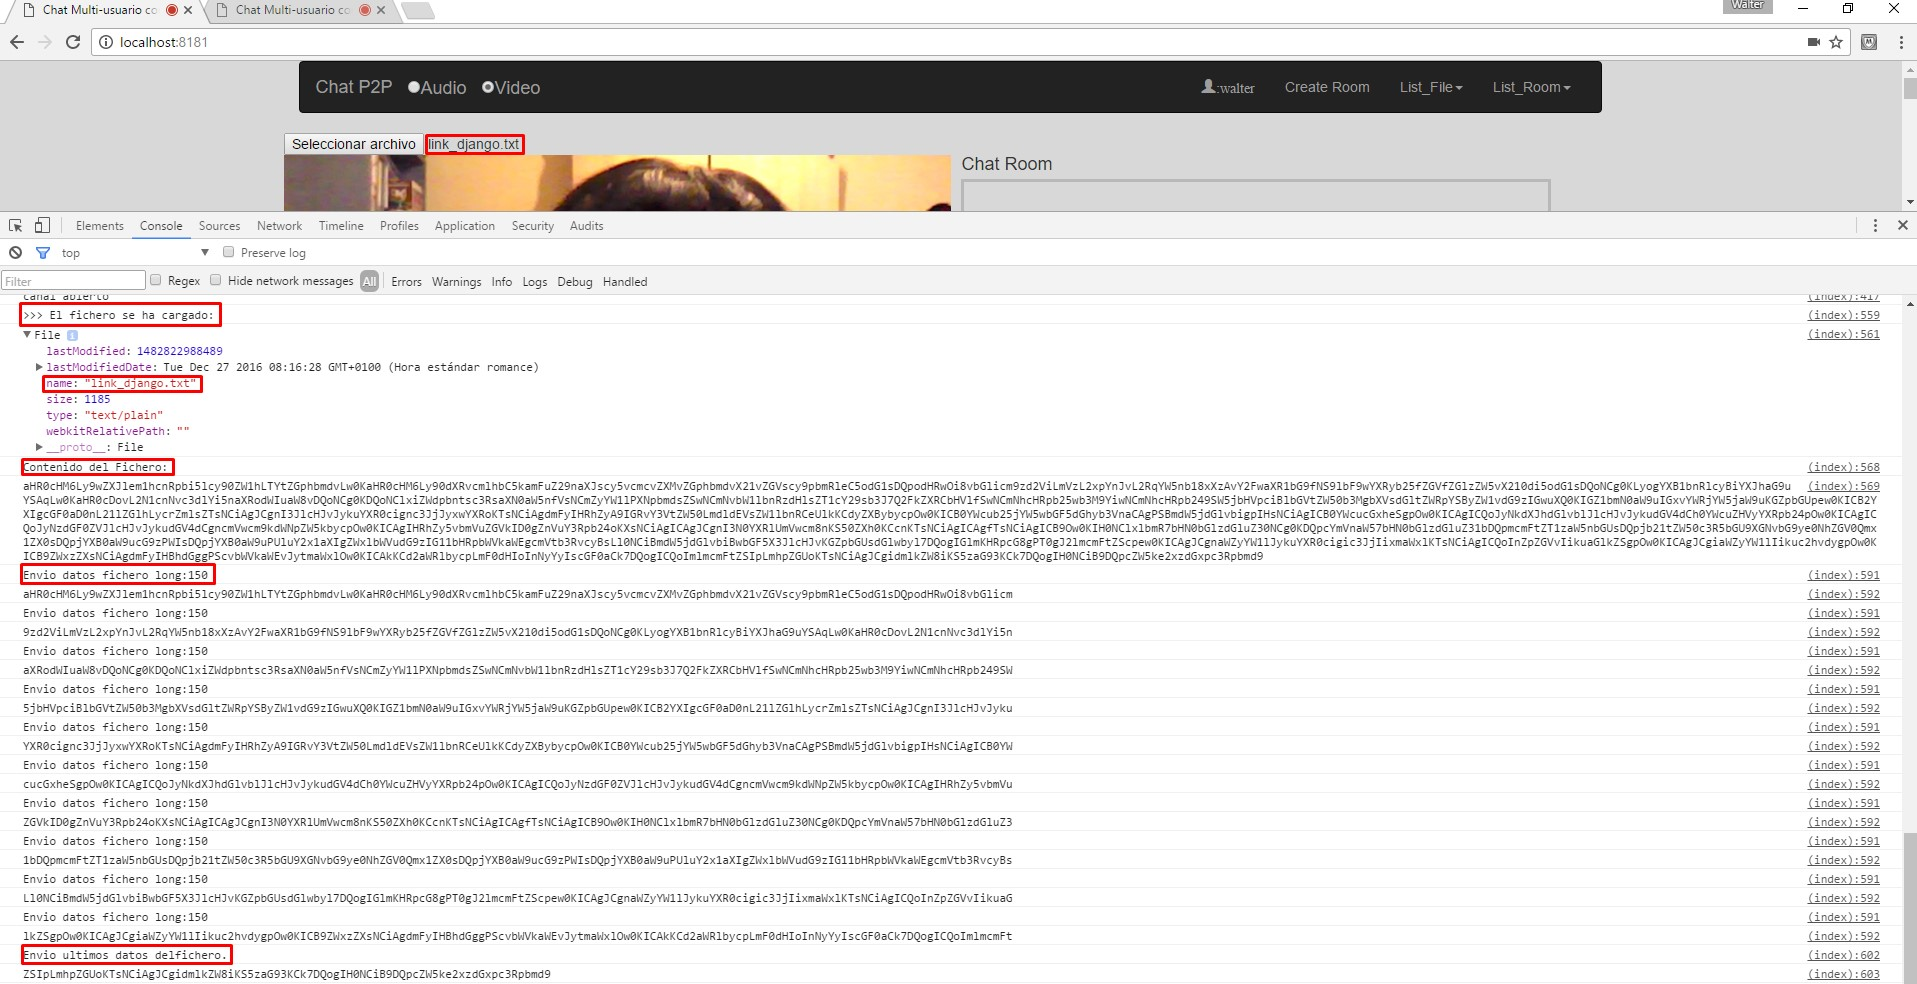
\includegraphics[width=0.7\linewidth]{Figures/filSendUser}
\decoRule
\caption[An Electron]{ComunnicacionWebRTC (artist's impression).}
\label{fig:fildSendUser}
\end{figure}
El usuario receptor ira acumulando cada uno de los fragmentos que reciba hasta obtener el ultimo fragmento mediante la función 'BuildField()'.Al obtener el ultimo fragmento pasmos a generar el documento a través una etiqueta '<a>' donde el atributo href esta formado por el tipo de archivo concadenado a los fragmentos del archivos(\textbf{fig \ref{fig:FieldReceiveUser}}).
\begin{lstlisting}[
frame=single,
commentstyle=\color{CadetBlue},
captionpos=b,
caption=Recepción y reconstrucción del fichero .]
 function BuildFile(_data) {
  blob += _data.data;
  if(_data.end != undefined){
   if(_data.more.type == 'text/plain'){
    var link = document.createElement('a');
    link.href = 'data:'+_data.more.type+';base64'+blob;
    link.target = '_blank';
    link.download = _data.more.name;
    var textnode = document.createTextNode(_data.more.name);
    link.appendChild(textnode);
    $("#listFile").append(link);
   }
   blob =',';
  }
 }  
\end{lstlisting}

\begin{figure}[!h]
\centering
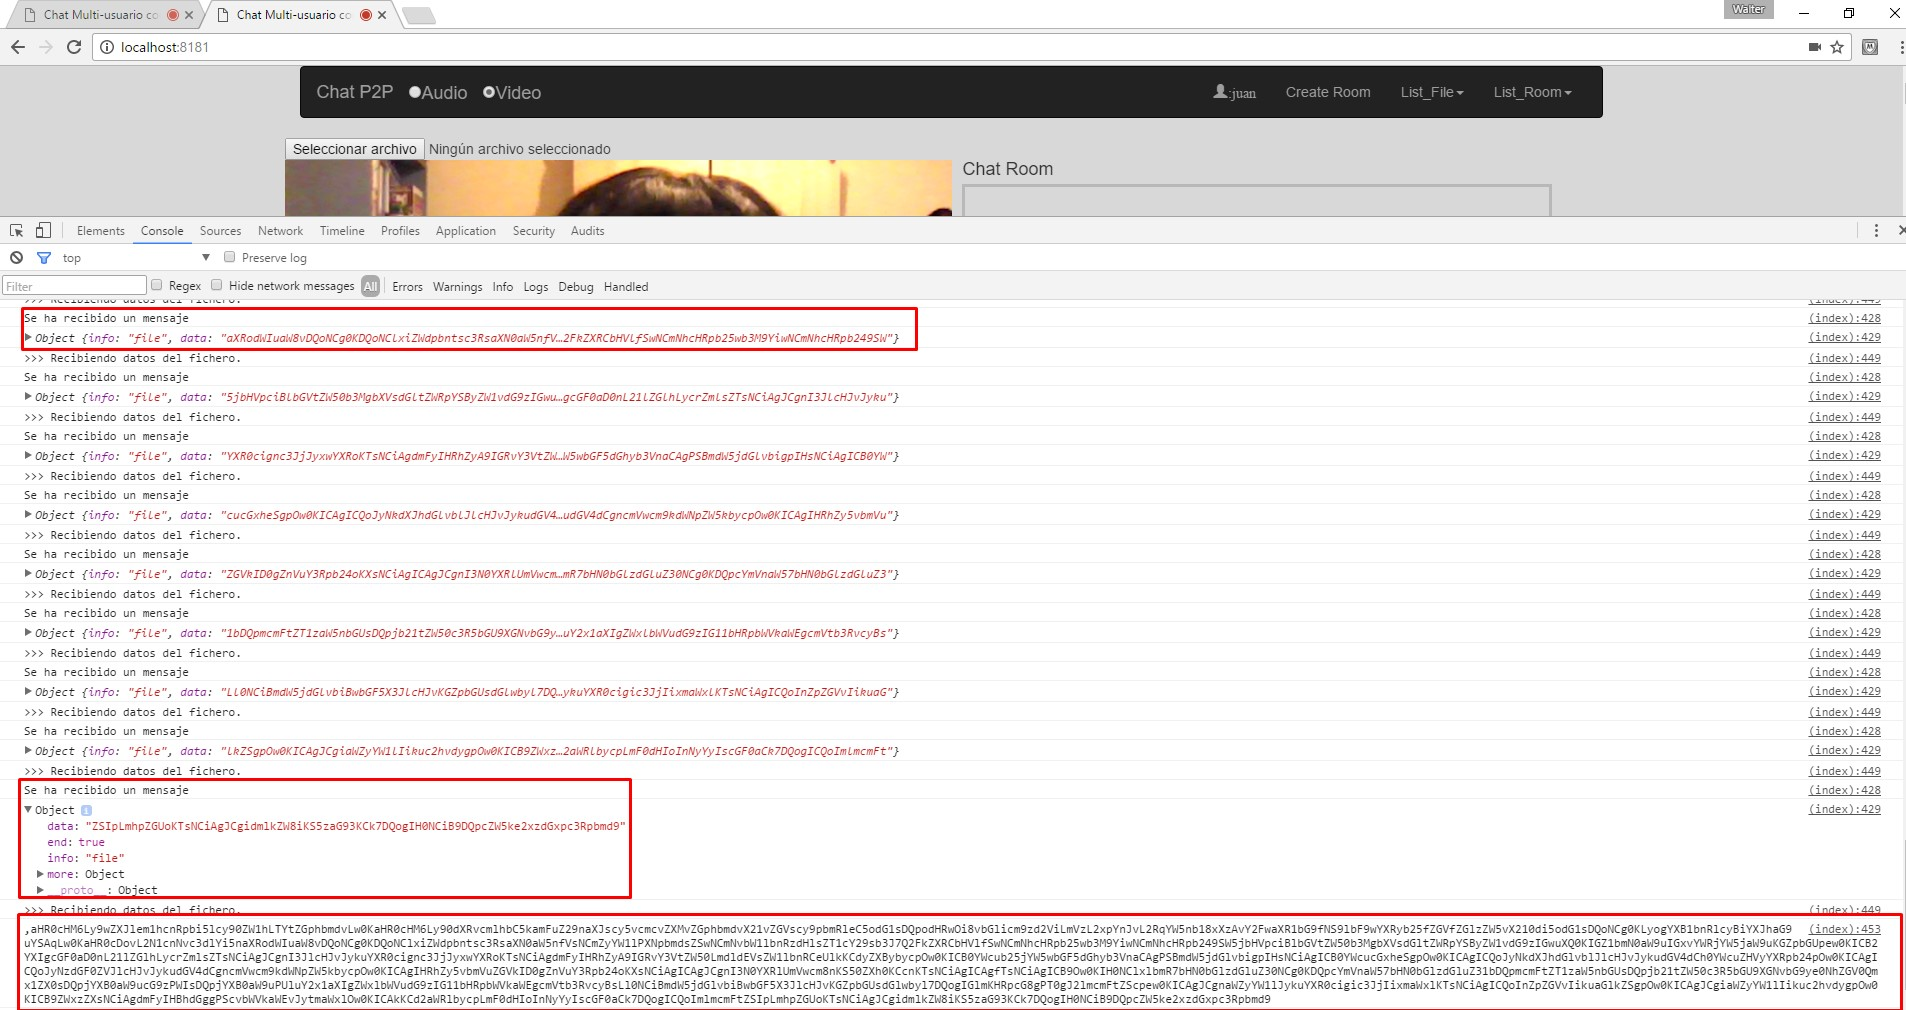
\includegraphics[width=0.7\linewidth]{Figures/filReceiveUser}
\decoRule
\caption[An Electron]{ComunnicacionWebRTC (artist's impression).}
\label{fig:FieldReceiveUser}
\end{figure}

\section{Pruebas}
